\documentclass[11pt,a4paper]{article}
\usepackage{amsmath,amssymb}
\usepackage[margin=2.5cm]{geometry}
\usepackage{array}
\usepackage{bm}
\usepackage{graphicx}
\usepackage{booktabs}
\usepackage{xcolor}
\usepackage{tikz}
\usetikzlibrary{arrows.meta,positioning,fit,backgrounds,calc}
\usepackage{hyperref}
\hypersetup{colorlinks=true, linkcolor=blue!50!black, citecolor=blue!50!black, urlcolor=blue!50!black}

% ---- tikz styles ----
\tikzset{
  block/.style={rectangle, rounded corners, draw=black!60, fill=blue!6,
    minimum height=9mm, minimum width=22mm, align=center, font=\small},
  frozen/.style={rectangle, rounded corners, draw=black!50, fill=black!7,
    minimum height=9mm, minimum width=22mm, align=center, font=\small},
  learn/.style={rectangle, rounded corners, draw=blue!60!black, fill=blue!14, very thick,
    minimum height=9mm, minimum width=22mm, align=center, font=\small},
  io/.style={rectangle, draw=black!40, fill=yellow!10, minimum height=8mm, align=center, font=\small},
  arr/.style={-{Stealth[length=2.2mm]}, thick},
}

\title{\textbf{Flow-Conditioned Metric 3D Point Tracking}\\[2pt]
\large SEA-RAFT optical flow $+$ Depth-Anything-3 metric depth $+$ a Mamba-3 depth refiner}
\author{Masahiro Ogawa}
\date{\today}

\begin{document}
\maketitle

\noindent
This note documents the \emph{methodology} and \emph{evaluation} of our 3D point tracker.
The system tracks query points in 3D over a monocular video by (i) propagating each query in 2D
with frozen SEA-RAFT optical flow~\cite{searaft}, (ii) lifting the 2D track to metric 3D with
frozen Depth-Anything-3 (DA3) metric depth~\cite{da3}, and (iii) refining only the per-point
\emph{depth along its (fixed) pixel ray} with a tiny causal Mamba-3 state-space model~\cite{mamba3}.
Evaluation is on TAPVid-3D~\cite{tapvid3d}, where we additionally introduce an
\emph{absolute-metric} protocol that exposes real-world depth quality hidden by the standard
scale-invariant leaderboard metric.

\tableofcontents

% =====================================================================
\section{Method}

\subsection{Overview}
Given a video $\{I_t\}_{t=1}^{F}$ and query points $\{(\mathbf{u}_n, a_n)\}_{n=1}^{N}$ (pixel
position $\mathbf{u}_n$ at anchor frame $a_n$), the goal is a 3D track
$\hat{\mathbf X}\in\mathbb{R}^{F\times N\times 3}$ and visibility $\hat v\in\{0,1\}^{F\times N}$.
Our pipeline (Fig.~\ref{fig:pipeline}) has a \emph{training-free} baseline --- SEA-RAFT
flow-chaining for the 2D track plus DA3 unprojection for 3D --- and a small \emph{learned} module,
v33, that refines depth.

\begin{figure}[h]
\centering
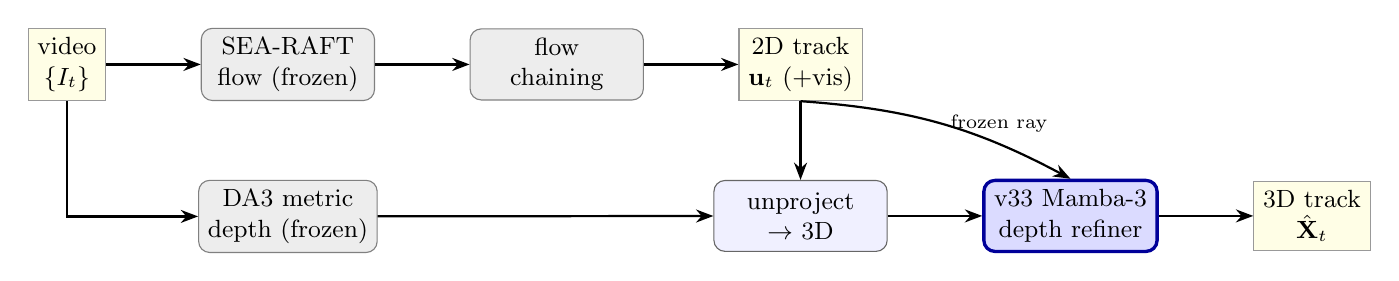
\begin{tikzpicture}[node distance=7mm and 12mm]
  \node[io] (vid) {video\\$\{I_t\}$};
  \node[frozen, right=of vid] (flow) {SEA-RAFT\\flow (frozen)};
  \node[frozen, right=of flow] (chain) {flow\\chaining};
  \node[io, right=of chain] (uv) {2D track\\$\mathbf{u}_t$ (+vis)};
  \node[frozen, below=10mm of flow] (da3) {DA3 metric\\depth (frozen)};
  \node[block, below=10mm of uv] (unp) {unproject\\$\to$ 3D};
  \node[learn, right=of unp] (v33) {v33 Mamba-3\\depth refiner};
  \node[io, right=of v33] (out) {3D track\\$\hat{\mathbf X}_t$};

  \draw[arr] (vid) -- (flow);
  \draw[arr] (flow) -- (chain);
  \draw[arr] (chain) -- (uv);
  \draw[arr] (vid.south) |- (da3.west);
  \draw[arr] (uv) -- (unp);
  \draw[arr] (da3) -- (unp);
  \draw[arr] (unp) -- (v33);
  \draw[arr] (v33) -- (out);
  \draw[arr] (uv.south) to[bend left=12] node[right,font=\scriptsize]{frozen ray} (v33.north);
\end{tikzpicture}
\caption{Pipeline. Grey = frozen / training-free; blue = the only learned module ($0.40$M params).
The 2D track and visibility from SEA-RAFT are \emph{never} modified; v33 refines depth along each
point's fixed pixel ray, so the 2D reprojection is invariant by construction (Fig.~\ref{fig:ray}).}
\label{fig:pipeline}
\end{figure}

\subsection{2D track: SEA-RAFT flow-chaining (baseline, frozen)}
We precompute dense forward/backward flow for consecutive frames with a frozen SEA-RAFT model,
$\mathbf{f}^{\rightarrow}_t,\mathbf{f}^{\leftarrow}_t$. Each query is propagated outward from its
anchor by bilinearly sampling the flow at the current position,
\begin{equation}
\mathbf{u}_{t+1} = \mathbf{u}_t + \mathcal{S}\!\left(\mathbf{f}^{\rightarrow}_t,\,\mathbf{u}_t\right),
\qquad
\mathbf{u}_{t-1} = \mathbf{u}_t + \mathcal{S}\!\left(\mathbf{f}^{\leftarrow}_{t-1},\,\mathbf{u}_t\right),
\end{equation}
where $\mathcal{S}$ is bilinear sampling. Visibility uses a forward--backward consistency test:
a hop is consistent iff $\lVert \mathbf{d}^{\rightarrow}+\mathbf{d}^{\leftarrow}\rVert \le
\alpha\,(\lVert\mathbf{d}^{\rightarrow}\rVert+\lVert\mathbf{d}^{\leftarrow}\rVert)+\beta$
($\alpha{=}0.05$, $\beta{=}1$\,px), and a point stays occluded once it fails. This 2D track is
strong on its own and is held \emph{fixed} for everything downstream.

\subsection{Metric depth and differentiable unprojection}
DA3 supplies a per-frame metric depth map $D_t$ (absolute metres). We sample it at the tracked
pixel and unproject with the pinhole intrinsics $K=(f_x,f_y,c_x,c_y)$:
\begin{equation}
z_t = \mathcal{S}(D_t,\mathbf{u}_t),\qquad
\hat{\mathbf X}_t = \Big(\tfrac{u_t-c_x}{f_x}\,z_t,\;\tfrac{v_t-c_y}{f_y}\,z_t,\;z_t\Big).
\label{eq:unproject}
\end{equation}
Sampling is done with \texttt{grid\_sample} so gradients flow to the (refined) depth; the depth
model itself is frozen. The baseline \emph{SEA-RAFT$+$DA3} tracker is exactly
Eq.~\eqref{eq:unproject} with $z_t$ taken directly from DA3.

\subsection{v33: Mamba-3 depth-along-ray refiner (the method)}
DA3 metric depth is accurate in \emph{relative} structure but carries a global scale bias
(e.g.\ $\sim$40\% on far-field driving scenes). v33 learns a small temporal correction to the
depth, leaving the 2D track untouched. The key design choice: with the pixel $\mathbf{u}_t$ frozen,
the only 3D degree of freedom that preserves the 2D reprojection is the depth $z_t$ along the pixel
ray (Fig.~\ref{fig:ray}).

\begin{figure}[h]
\centering
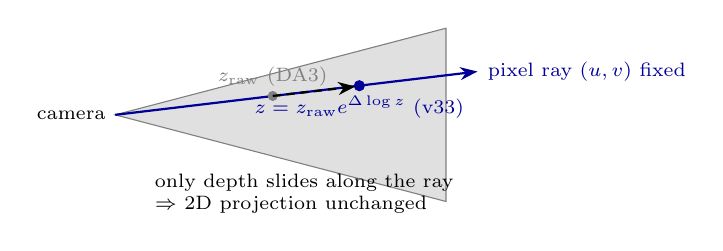
\begin{tikzpicture}[scale=1.0]
  \coordinate (cam) at (0,0);
  \draw[fill=black!12,draw=black!50] (cam) -- (4.2,1.1) -- (4.2,-1.1) -- cycle;
  \node[font=\scriptsize,left] at (cam) {camera};
  \draw[arr,blue!60!black,thick] (cam) -- (4.6,0.55) node[right,font=\scriptsize]{pixel ray $(u,v)$ fixed};
  \filldraw[gray] (2.0,0.24) circle (1.6pt) node[above,font=\scriptsize]{$z_{\text{raw}}$ (DA3)};
  \filldraw[blue!60!black] (3.1,0.37) circle (1.8pt) node[below,font=\scriptsize]{$z=z_{\text{raw}}e^{\Delta\log z}$ (v33)};
  \draw[arr,densely dashed] (2.0,0.24) -- (3.05,0.36);
  \node[font=\scriptsize,align=left] at (2.4,-1.0)
    {only depth slides along the ray\\$\Rightarrow$ 2D projection unchanged};
\end{tikzpicture}
\caption{Depth-along-ray refinement. The tracked pixel (hence the ray direction) is frozen;
v33 only moves the point's depth, so the predicted 2D track and visibility are invariant.}
\label{fig:ray}
\end{figure}

\paragraph{Inputs and architecture.} For each track $n$ and frame $t$ the model sees a $4$-D
feature: the normalised ray direction $\big(\tfrac{u-c_x}{f_x},\tfrac{v-c_y}{f_y}\big)$, the raw
depth $z_{\text{raw}}/z_{\text{ref}}$ ($z_{\text{ref}}=$ per-clip median depth), and the visibility
flag. An MLP embeds this to $D{=}128$; two \emph{causal} Mamba-3 layers process each track as a
length-$F$ temporal sequence; a zero-initialised head emits a log-depth correction
(Fig.~\ref{fig:arch}):
\begin{equation}
\Delta\log z_t = \mathrm{clamp}\big(\mathrm{head}(h_t),\,\pm 2\big),\qquad
z_t = z_{\text{raw},t}\cdot e^{\Delta\log z_t},
\end{equation}
and the 3D point is reprojected with Eq.~\eqref{eq:unproject} using the refined $z_t$ and the
\emph{frozen} ray. Zero-init means v33 starts exactly at the SEA-RAFT$+$DA3 baseline and only learns
improvements. The model has $\approx0.40$M trainable parameters.

\begin{figure}[h]
\centering
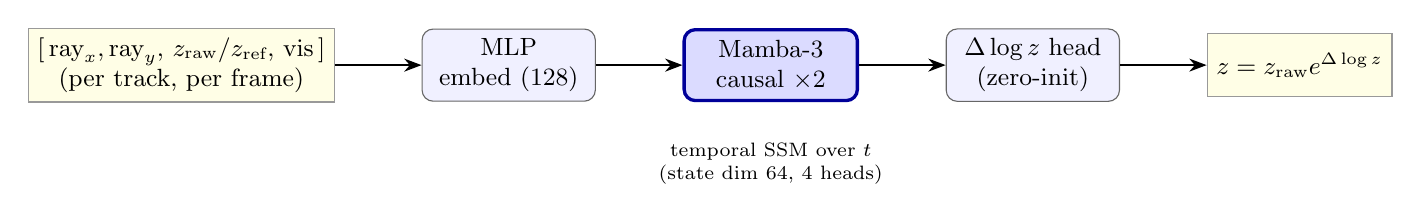
\begin{tikzpicture}[node distance=6mm and 11mm]
  \node[io] (in) {$[\,\text{ray}_x,\text{ray}_y,\,z_{\text{raw}}/z_{\text{ref}},\,\text{vis}\,]$\\(per track, per frame)};
  \node[block, right=of in] (emb) {MLP\\embed (128)};
  \node[learn, right=of emb] (m1) {Mamba-3\\causal $\times 2$};
  \node[block, right=of m1] (head) {$\Delta\log z$ head\\(zero-init)};
  \node[io, right=of head] (z) {$z=z_{\text{raw}}e^{\Delta\log z}$};
  \draw[arr] (in) -- (emb);
  \draw[arr] (emb) -- (m1);
  \draw[arr] (m1) -- (head);
  \draw[arr] (head) -- (z);
  \node[font=\scriptsize, below=4mm of m1, align=center] {temporal SSM over $t$\\(state dim 64, 4 heads)};
\end{tikzpicture}
\caption{v33 architecture. Each of the $N$ tracks is processed independently as a temporal
sequence by the causal Mamba-3 stack; the head outputs a bounded multiplicative depth correction.}
\label{fig:arch}
\end{figure}

\subsection{Why depth-only (and not 2D)}
An earlier variant (v32) added a learned 2D residual $\Delta\mathbf{u}$ on top of SEA-RAFT. It
\emph{degraded} accuracy: SEA-RAFT's 2D track is already near-optimal, and small nudges push the
sampling location across DA3 depth discontinuities (object boundaries), flipping points out of the
correctness band. v33 therefore freezes the 2D track entirely and refines depth only --- the lever
that actually carries the error.

\subsection{Training}
Only the $0.40$M-parameter refiner is trained. The loss is 3D-position-only (the 2D track and
visibility are frozen, so they carry no gradient):
\begin{equation}
\mathcal{L} = \frac{1}{|\mathcal{V}|}\sum_{(t,n)\in\mathcal{V}}
\frac{\lVert \hat{\mathbf X}_{t,n}-\mathbf X^{*}_{t,n}\rVert_1}{s_{\text{clip}}},
\end{equation}
an $\ell_1$ error over visible points, normalised by the per-clip median anchor-frame depth
$s_{\text{clip}}$ (matching the benchmark's scale convention). We train $20$k steps (AdamW,
lr $3\!\times\!10^{-4}$, warmup $500$, $8$-frame windows, bf16; $\sim$9.5\,h on one GPU).

% =====================================================================
\section{Evaluation}

\subsection{Protocol and metrics}
We evaluate on the TAPVid-3D~\cite{tapvid3d} \textbf{minival} split (150 clips: 50 each of
\emph{pstudio} indoor mocap $\sim$3\,m, \emph{drivetrack} driving $\sim$20\,m, \emph{adt} egocentric
$\sim$1\,m). The headline metric is 3D Average Jaccard (3D-AJ), combining within-threshold position
accuracy and occlusion. Crucially, the official 3D-AJ is \emph{scale-invariant twice over}: (i) it
rescales the predicted cloud by the per-clip median $\lVert\mathbf X^{*}\rVert/\lVert\hat{\mathbf X}\rVert$
before scoring, and (ii) its within-threshold radii are depth-relative pixel thresholds (referenced
to $256$-px images). Both choices discard absolute depth --- exactly the quantity that matters for
metric 3D reconstruction.

We therefore additionally report an \textbf{absolute-metric} protocol: the same official metric with
\emph{no} median scaling and \emph{fixed metre} thresholds ($1$\,cm$\,\ldots\,2.56$\,m), giving
metric-AJ and metric-APD3D, plus the mean/median 3D error in metres. Our pipeline reproduces the
official scale-invariant metric exactly (we recover SpatialTracker's published drivetrack 3D-AJ of
$0.058$ to three decimals once the $256$-px intrinsics convention is applied), so the absolute
variant is a faithful, scale-sensitive extension rather than a re-implementation.

\subsection{Leaderboard (scale-invariant) results}
Table~\ref{tab:median} reports median-scaled 3D-AJ. The training-free SEA-RAFT$+$DA3 baseline
already matches or exceeds the 2024 published baselines\footnote{We use 2025 components
(DA3-Metric-Large depth); the published baselines use 2024 depth (ZoeDepth) / SfM. A final
official cross-check on our \emph{own} saved predictions is pending, but the pipeline is validated
by exactly reproducing the SpatialTracker number.}, while v33 \emph{loses} on this metric (it
trades relative-structure quality for absolute-scale correctness; see \S\ref{sec:abs}). Current
state-of-the-art on the (different, larger) full-eval split is far higher --- TAPIP3D $\sim$0.30 ---
and a head-to-head against it is in progress (\S\ref{sec:sota}).

\begin{table}[h]
\centering
\caption{TAPVid-3D minival, median-scaled 3D-AJ (the standard leaderboard metric; higher better).}
\label{tab:median}
\begin{tabular}{lrrrr}
\toprule
Method & pstudio & drivetrack & adt & mean \\
\midrule
BootsTAPIR + ZoeDepth (2024)\,$^{*}$ & 0.102 & 0.051 & 0.086 & 0.080 \\
SpatialTracker (2024)\,$^{*}$        & 0.098 & 0.058 & 0.092 & 0.083 \\
\midrule
SEA-RAFT + DA3 (baseline, no training) & 0.111 & 0.108 & 0.132 & \textbf{0.117} \\
v33 (depth refiner)                    & 0.041 & 0.057 & 0.123 & 0.074 \\
\bottomrule
\end{tabular}
\\[2pt]
{\footnotesize $^{*}$ published numbers; entire leaderboard is median-scaled.}
\end{table}

\subsection{Absolute-metric results: the reversal}
\label{sec:abs}
Under the absolute-metric protocol the ranking \emph{reverses} (Table~\ref{tab:abs},
Fig.~\ref{fig:reversal}). v33 beats the baseline on every absolute measure overall: metric-AJ
$+22\%$, metric-APD3D $+20\%$, mean error $-38\%$ ($4.29\!\to\!2.67$\,m), median error $-47\%$. The
gain is concentrated where DA3's scale is most wrong --- far-field \emph{drivetrack}, metric-AJ
$0.005\!\to\!0.082$ ($16\times$), error $11.7\!\to\!6.9$\,m --- while near-field \emph{adt}
(already accurate) is a tie. The learned corrector helps exactly when needed and does no harm
otherwise; the leaderboard's median scaling hides all of this.

\begin{table}[h]
\centering
\caption{TAPVid-3D minival. ``median-AJ'' is the leaderboard metric; ``metric-*'' and the error
columns are absolute (no scaling, fixed-metre thresholds). Both methods run at $\sim$12.5 fps.}
\label{tab:abs}
\begin{tabular}{lrrrrr}
\toprule
Method & median-AJ & metric-AJ & metric-APD3D & err mean (m) & err med (m) \\
\midrule
SEA-RAFT + DA3 (baseline) & \textbf{0.117} & 0.147 & 0.254 & 4.29 & 4.01 \\
v33 (depth refiner)       & 0.074 & \textbf{0.180} & \textbf{0.306} & \textbf{2.67} & \textbf{2.13} \\
\bottomrule
\end{tabular}
\end{table}

\begin{figure}[h]
\centering
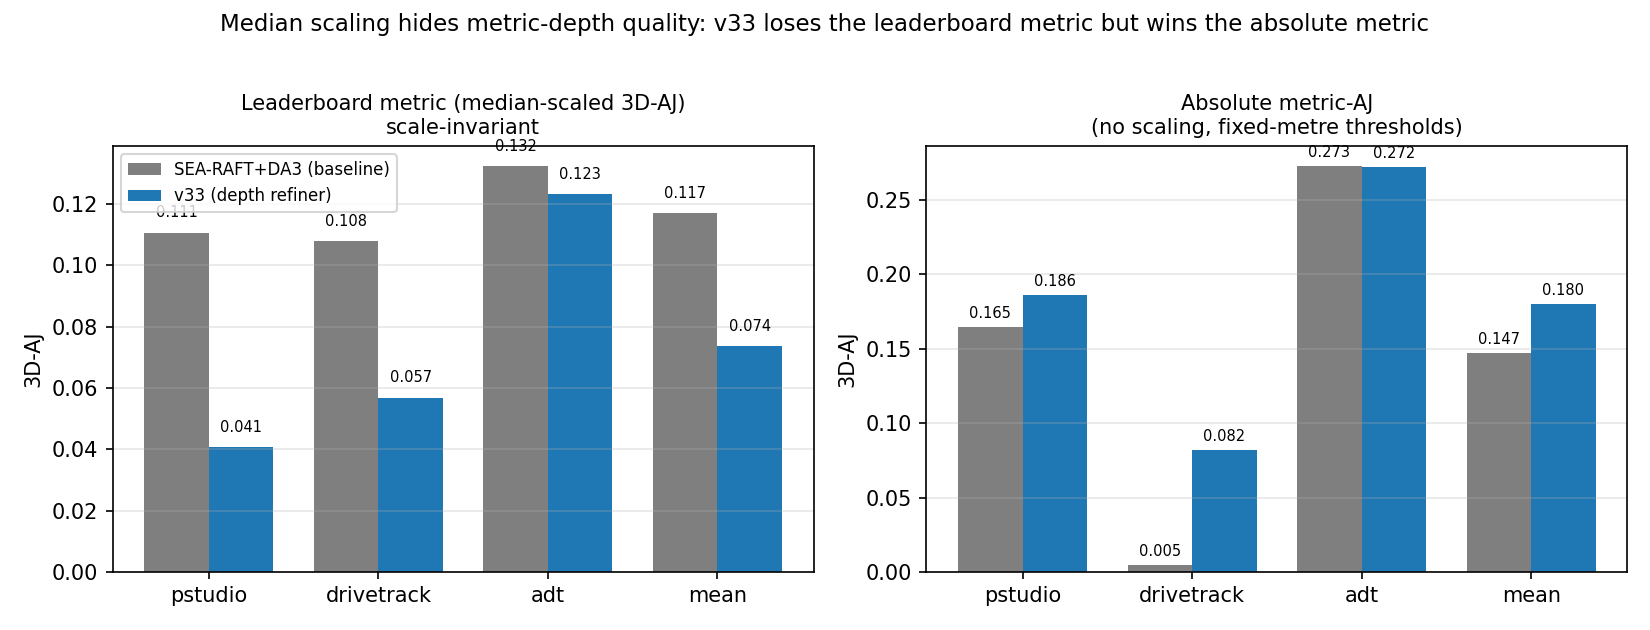
\includegraphics[width=\textwidth]{figs/fig_metric_reversal.png}
\caption{Median scaling hides metric-depth quality. Left: the scale-invariant leaderboard 3D-AJ
favours the baseline. Right: under the absolute metric, v33 wins --- most on far-field drivetrack.}
\label{fig:reversal}
\end{figure}

\subsection{Comparison to SOTA (drivetrack)}
\label{sec:sota}
SpatialTracker's official predictions are released only for \emph{drivetrack}. Scored identically
through our pipeline (and validated: its median-scaled 3D-AJ reproduces the published $0.058$),
v33 \emph{beats} this SOTA 3D tracker in absolute metric on drivetrack (Fig.~\ref{fig:sota}):
metric-AJ $0.082$ vs $0.069$ ($+20\%$), metric-APD3D $0.134$ vs $0.106$ ($+26\%$), median error
$5.50$ vs $6.03$\,m. A comparison against the current SOTA TAPIP3D (image-only, DA3 depth ---
a fair, metric-depth-grounded baseline) is \textbf{in progress}: its per-clip predictions will be
scored with the same protocol via our external-prediction ingestion.

\begin{figure}[h]
\centering
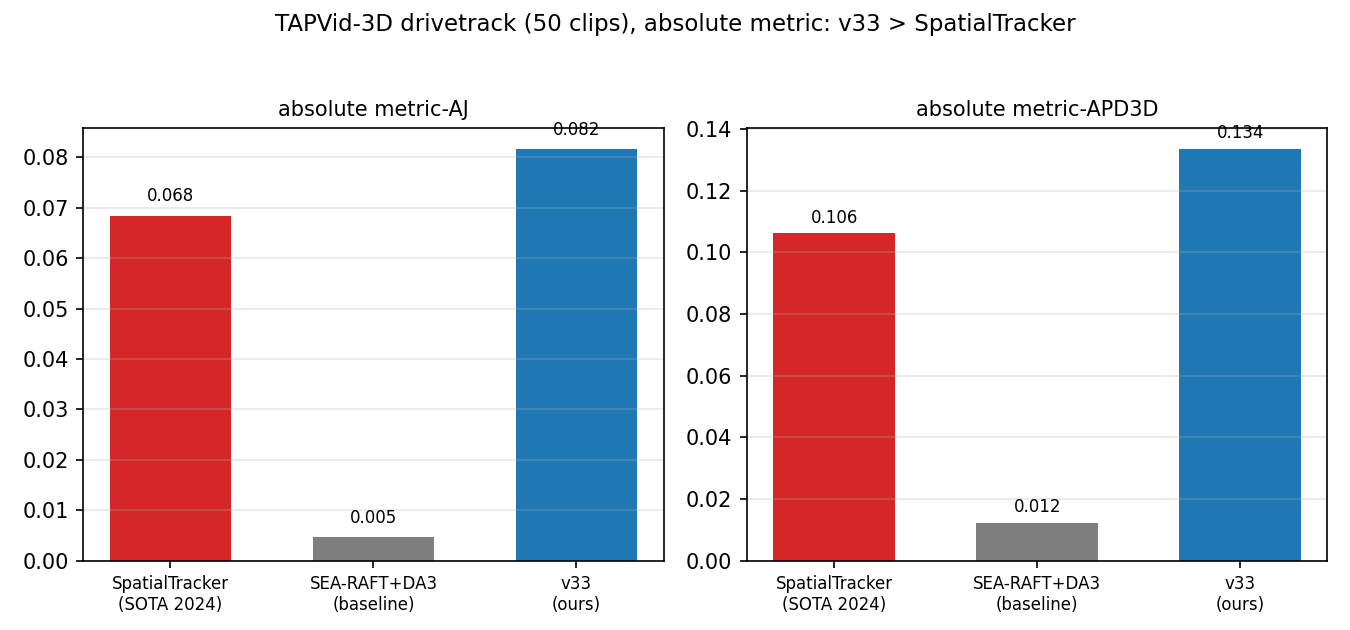
\includegraphics[width=0.85\textwidth]{figs/fig_sota_drivetrack.png}
\caption{Drivetrack (50 clips), absolute metric. v33 outperforms the 2024 SOTA SpatialTracker and
the training-free baseline.}
\label{fig:sota}
\end{figure}

\subsection{Qualitative results}
Figures~\ref{fig:qual-pstudio}--\ref{fig:qual-adt} show predicted (solid) vs ground-truth (dashed)
3D trajectories, baseline vs v33, one clip per subset. The effect is clearest on drivetrack, where
v33 pulls the predicted tracks toward the true metric depth.

\begin{figure}[h]
\centering
\begin{minipage}{0.49\textwidth}\centering
  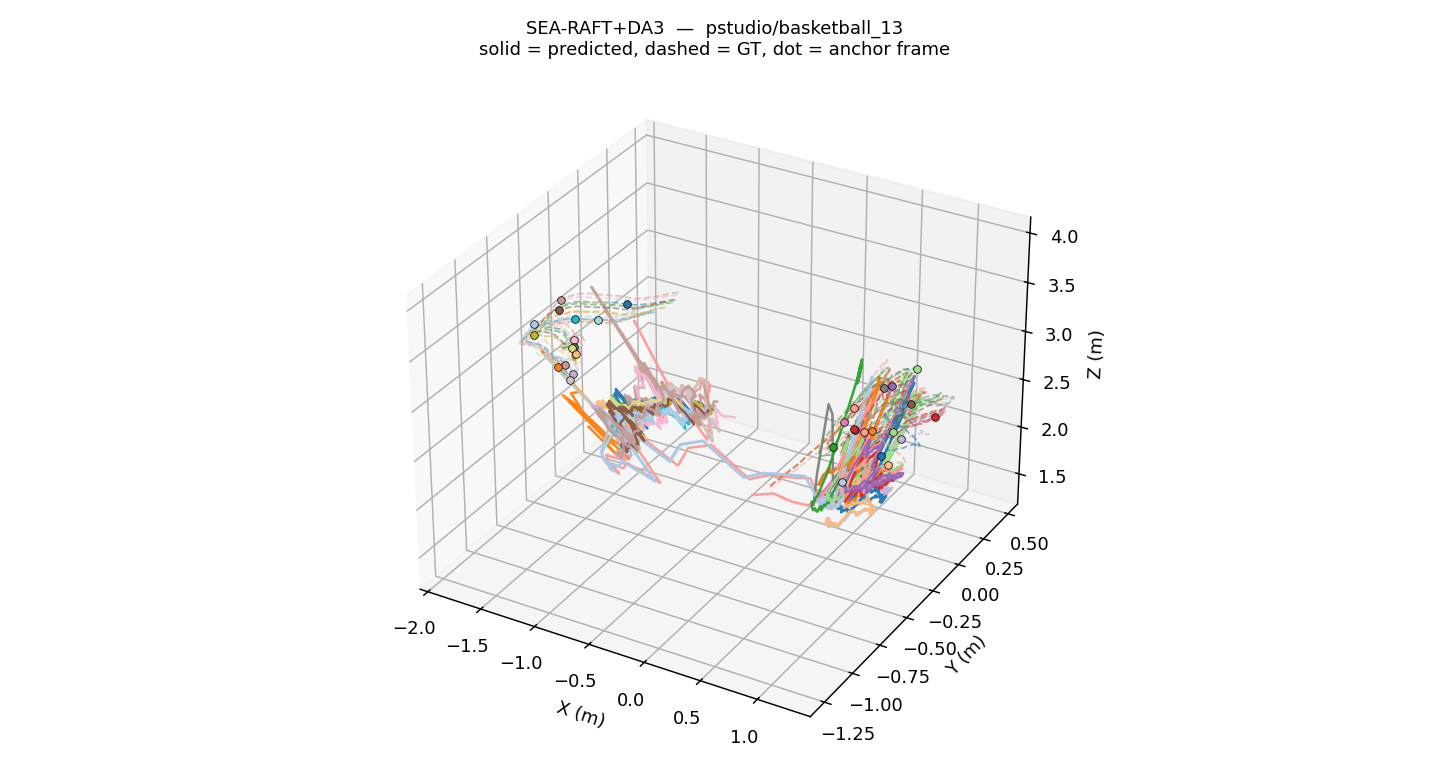
\includegraphics[width=\textwidth]{figs/qual_pstudio_baseline_3d.png}\\{\footnotesize baseline}
\end{minipage}\hfill
\begin{minipage}{0.49\textwidth}\centering
  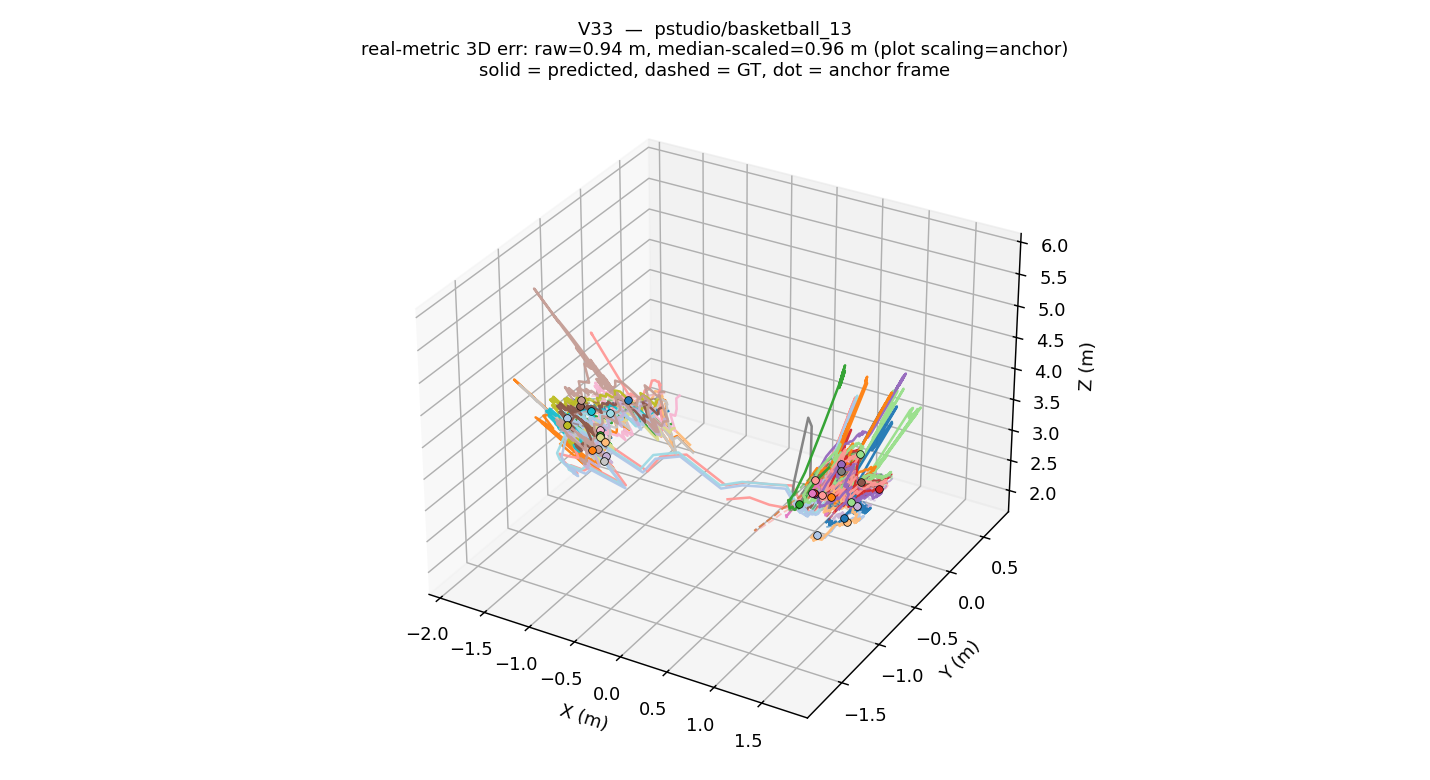
\includegraphics[width=\textwidth]{figs/qual_pstudio_v33_3d.png}\\{\footnotesize v33}
\end{minipage}
\caption{pstudio (indoor, $\sim$3\,m): 3D trajectories, baseline vs v33.}
\label{fig:qual-pstudio}
\end{figure}

\begin{figure}[h]
\centering
\begin{minipage}{0.49\textwidth}\centering
  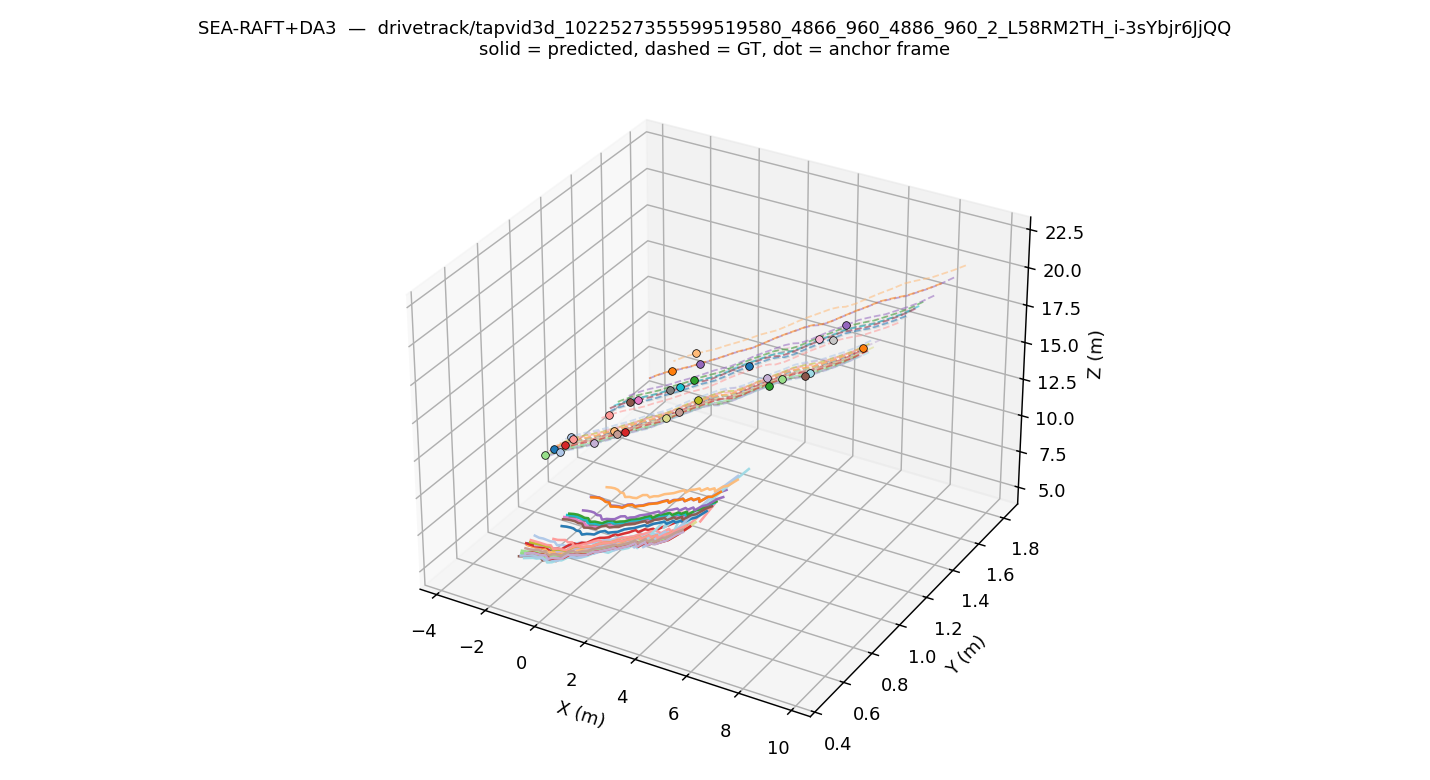
\includegraphics[width=\textwidth]{figs/qual_drivetrack_baseline_3d.png}\\{\footnotesize baseline}
\end{minipage}\hfill
\begin{minipage}{0.49\textwidth}\centering
  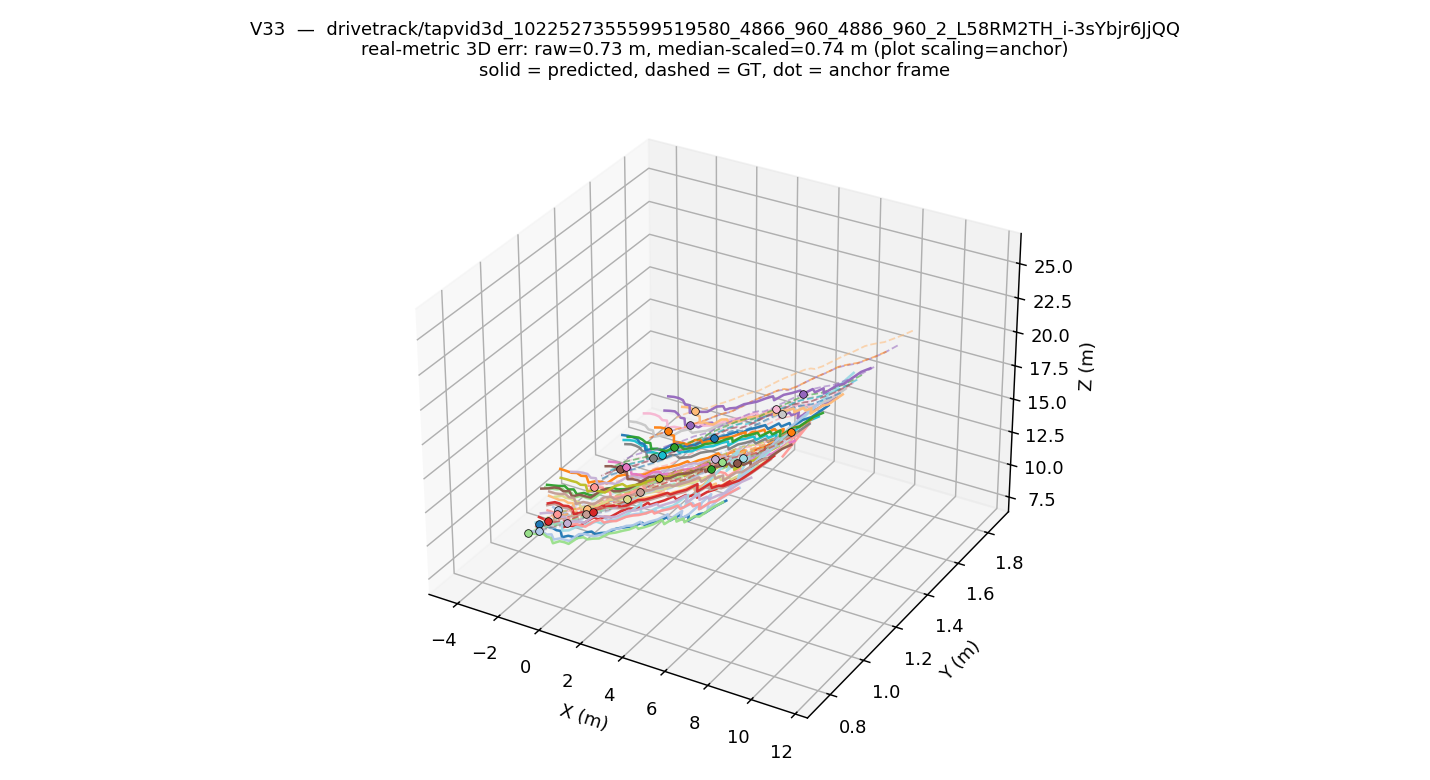
\includegraphics[width=\textwidth]{figs/qual_drivetrack_v33_3d.png}\\{\footnotesize v33}
\end{minipage}
\caption{drivetrack (driving, $\sim$20\,m): the far-field scene where v33's depth correction helps most.}
\label{fig:qual-drivetrack}
\end{figure}

\begin{figure}[h]
\centering
\begin{minipage}{0.49\textwidth}\centering
  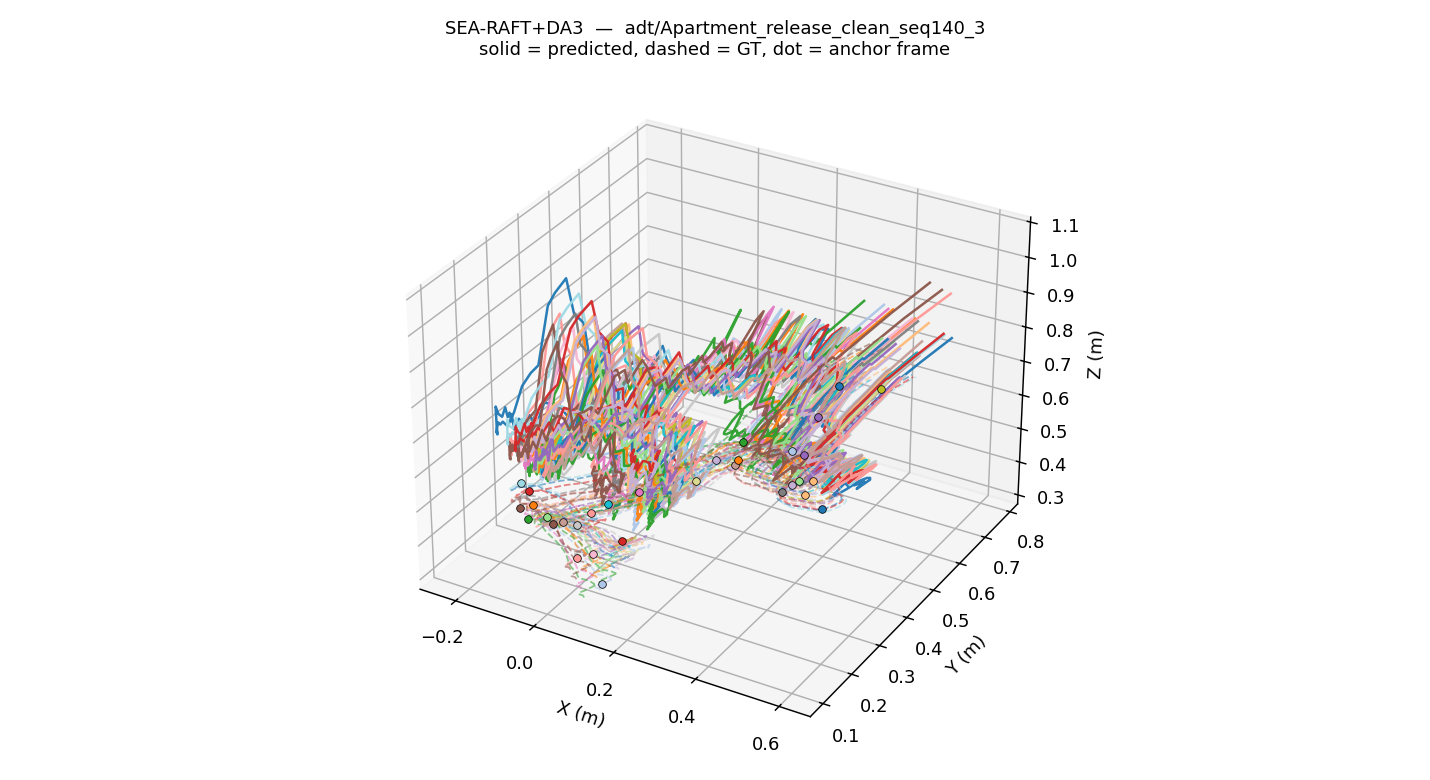
\includegraphics[width=\textwidth]{figs/qual_adt_baseline_3d.png}\\{\footnotesize baseline}
\end{minipage}\hfill
\begin{minipage}{0.49\textwidth}\centering
  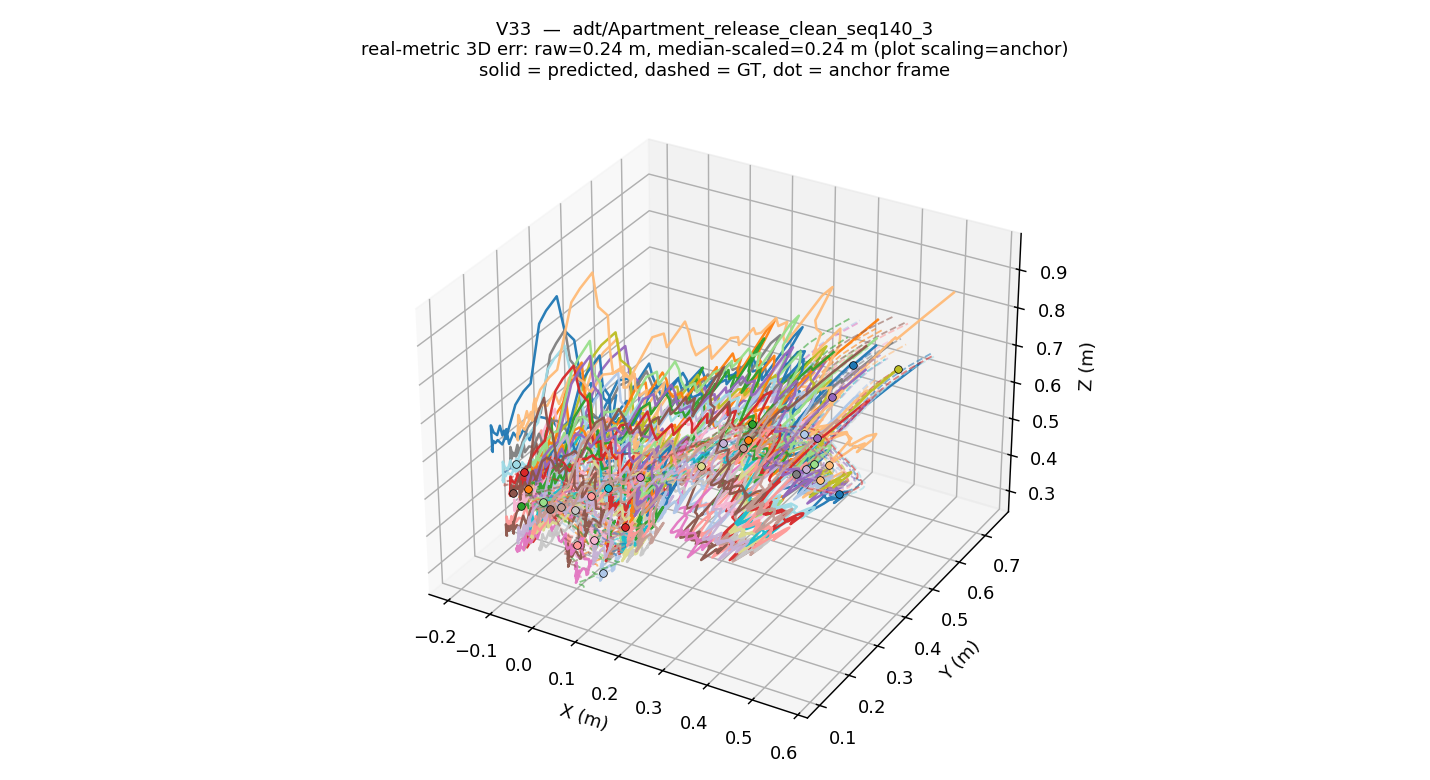
\includegraphics[width=\textwidth]{figs/qual_adt_v33_3d.png}\\{\footnotesize v33}
\end{minipage}
\caption{adt (egocentric, $\sim$1\,m): near-field, where DA3 is already accurate (tie).}
\label{fig:qual-adt}
\end{figure}

\begin{figure}[h]
\centering
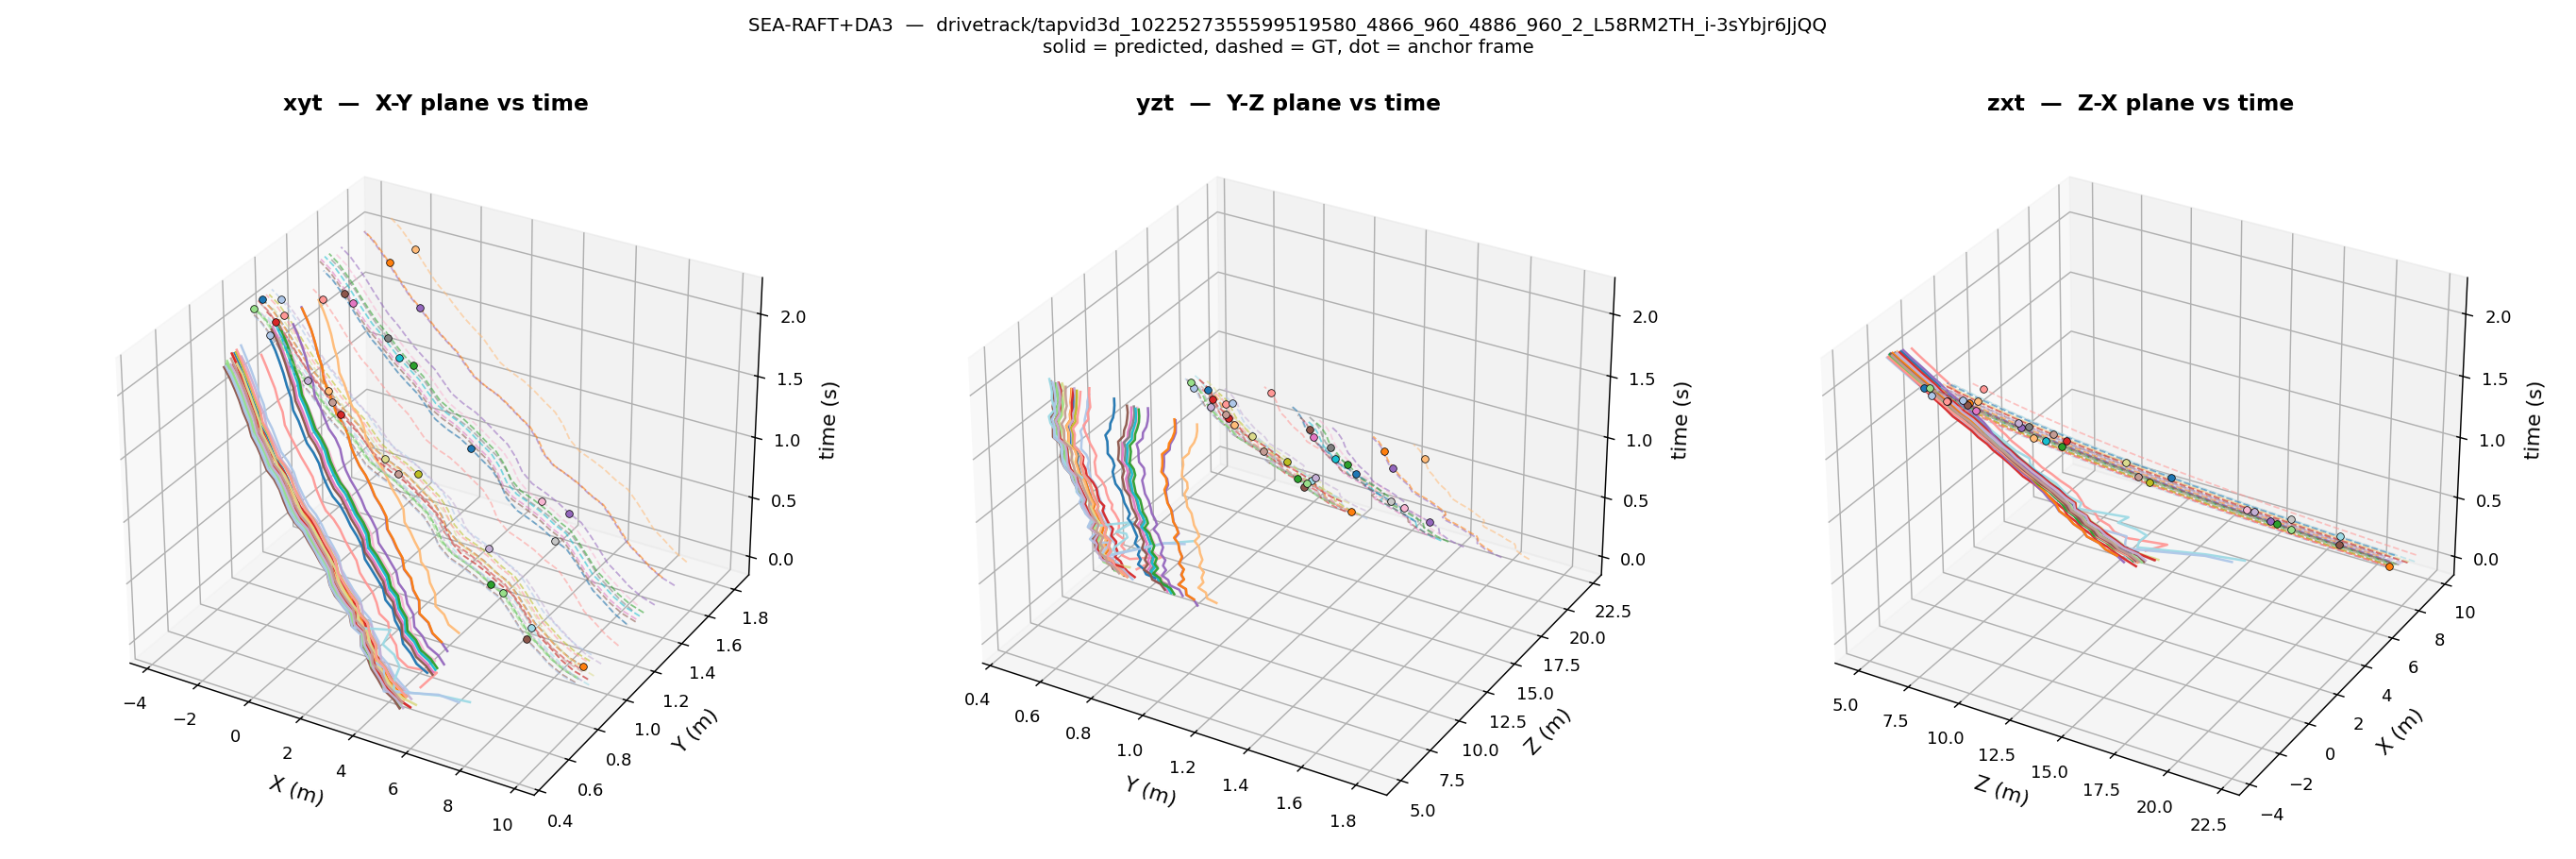
\includegraphics[width=0.92\textwidth]{figs/qual_drivetrack_baseline_st.png}
\caption{Space-time view (drivetrack baseline): per-axis position over time, $X$-$t$/$Y$-$t$/$Z$-$t$,
predicted (solid) vs ground truth (dashed).}
\label{fig:qual-st}
\end{figure}

\subsection{Efficiency}
\begin{table}[h]
\centering
\caption{Efficiency. v33 adds a $0.40$M-param refiner with negligible cost over the baseline.}
\begin{tabular}{lrr}
\toprule
Method & throughput (fps) & trainable params \\
\midrule
SEA-RAFT + DA3 (baseline) & 12.4 & 0 \\
v33 (depth refiner)       & 12.5 & 0.40\,M \\
\bottomrule
\end{tabular}
\end{table}

% =====================================================================
\begin{thebibliography}{9}
\bibitem{tapvid3d} Koppula et al., \textit{TAPVid-3D: A Benchmark for Tracking Any Point in 3D}, NeurIPS 2024.
\bibitem{searaft} Wang et al., \textit{SEA-RAFT: Simple, Efficient, Accurate RAFT for Optical Flow}, ECCV 2024.
\bibitem{da3} \textit{Depth-Anything-3: metric monocular depth/geometry}, 2025.
\bibitem{mamba3} \textit{Mamba-3 / structured state-space duality}, 2024--2025.
\bibitem{spatialtracker} Xiao et al., \textit{SpatialTracker: Tracking Any 2D Pixels in 3D Space}, CVPR 2024.
\bibitem{tapip3d} \textit{TAPIP3D: Tracking Any Point in Persistent 3D Geometry}, 2025.
\end{thebibliography}

\end{document}
